\chapter{基礎知識}
\cout{
本章では,本論文で扱うProgrammable Microfluidic Device(PMD)というバイオチップの基礎知識についての説明をする.
まず,PMDのアーキテクチャについて説明する.
そして,PMDのアーキテクチャの欠点についても説明する.
最後に,既存手法として,PMDのアーキテクチャの欠点に対応したPMD上での混合手順の生成手法
No Transport Mixing(NTM)について簡単に説明する.}
\section{PMD}
\cout{この節では,PMDというデバイスがどういったアーキテクチャを持つかを説明する.}
\subsection{PMDのアーキテクチャ}
\label{ark}
%PMDとはどういうデバイスか説明を書く.
\cout{
PMDの顕微鏡写真を図~\ref{fig:micrograph}に示した~\cite{1}.
図~\ref{fig:micrograph}において,赤黒く見えるのはバルブという部品で,バルブによって囲まれていて青い線の交点と重なっている領域はセルと呼ばれる.
バルブは開閉の操作を行うことが可能である.
図~\ref{fig:mixing}では,PMDに流し込まれた試薬が混合される様子を表している~\cite{4}.
図~\ref{fig:mixing}(a)から(b)は,圧力をかけられることで試薬が入力ポートからPMDの内部へと流入する様子を表している.
図~\ref{fig:mixing}(c)は,バルブの開閉の制御によって,ミキサーと呼ばれるセルが円環状に繋げられた流路が生成される様子を表している.
ミキサー内のバルブの開閉を行うことにより,ミキサー内の液滴の混合が行われる.
そして,液滴の混合の後は,図~\ref{fig:mixing}(d)で表されているようにミキサー内のどのセルにおいても格納されている液滴の濃度は等しくなる.
}

\cout{
    また,PMDでは,開閉するバルブの組み合わせを変えることにより,図~\ref{fig:4and6Mixer}で表したような様々な大きさのミキサーを生成することもできる.
    図~\ref{fig:4and6Mixer}(a)は2$\times2$のセルを用いる2$\times2$ミキサー,図~\ref{fig:4and6Mixer}(b)は2$\times$3セルを用いる2$\times$3ミキサーである.
    PMDに収まる限り,これら以外にも様々な大きさのミキサーの生成,及び,そのミキサー上での試薬の混合が可能である.
}
\begin{figure}[tbp]
 \centering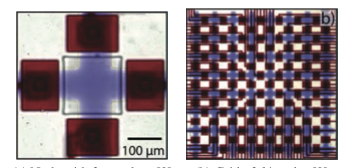
\includegraphics[scale=1.0]{img/PMDMicrograph.pdf}
 \caption{PMDの顕微鏡写真,参考文献~\cite{1}より引用}\label{fig:micrograph}
\end{figure}
\begin{figure}[tbp]
 \centering\includegraphics[scale=0.8]{img/PMDMixing_jp.pdf}
    \caption{PMD上に流し込まれた2種類の試薬が混合される様子,参考文献~\cite{4}より引用し一部改変}\label{fig:mixing}
\end{figure}
\begin{figure}[tbp]
    \centering\includegraphics[scale=0.5]{img/4and6Mixer.pdf}
 \caption{PMDで生成可能なミキサー}\label{fig:4and6Mixer}
\end{figure}
\newpage
\subsection{PMDにおけるセル間の液滴の移動}
%既存手法の説明への前提知識として,PMDにおいてセル間での液滴の移動操作は原則不可能であるということを説明する.
\cout{
    バイオチップの中心的なアーキテクチャであるDMFB(Digital Microfluid biochip)においては,PMDでのセルに相当する電極の間での試薬の移動操作~\cite{B110474H}を用い,試薬合成が行われる~\cite{5605330}\cite{10.1007/s11047-006-9032-6}\cite{10.1145/2429384.2429464}.
それに対して,PMDでは,セル間での液滴の移動操作は原則的に不可能であることが知られている.
図~\ref{fig:fluidseg}はセル間での液滴を移動を試みる前と後のPMDの状態を表している~\cite{4}. 
図~\ref{fig:fluidseg}(a)は,始点セルに格納されている液滴の目標セルへの移動を試みる前の状態を表している.
そして,
図~\ref{fig:fluidseg}(b)は,油のみを通すマイクロ流体ラッチ~\cite{urbanski2006digital}と油を用いて始点セルに配置された液滴の目標セルへの移動を試みた後の様子が表されている.
圧力をかけて互いに混ざらない液滴と油を移動させようとすると,移動経路上の直角部分で液滴にかかる力が部分ごとに均一でなくなり,\mbox{図~\ref{fig:fluidseg}(b)}のような液滴の分割が発生する~\cite{FU2015343}.
}

\cout{
以上で述べたように,経路上において液滴の分割が発生するため,PMDにおけるセル間の液滴の移動操作は不可能である.
したがって,PMDで試薬合成を行うためには,セル間での液滴移動のない混合手順を生成する必要がある.
}
\begin{figure}[tbp]
    \centering\includegraphics[scale=0.8]{img/FluidSegmentation_jp.pdf}
 \caption{fluid segmentationの様子,参考文献~\cite{4}より引用し一部改変}\label{fig:fluidseg}
\end{figure}
\newpage
\section{{2×2ミキサーを用いた液滴移動の\bout{ない}混合手順の生成}}
%セル間の液滴の移動操作を必要としない試薬混合手法NTM(No Transport Mixing)の説明をする.
%その後,既存の希釈木のNTMでのPMDへのマッピング手法を説明する.
\cout{
    前述した通り,PMDで試薬合成を行うためには,セル間での液滴移動のない混合手順を生成する必要がある.
    したがって,本節ではPMD上でのセル間の液滴移動のない混合手順の生成の既存手法であるNTM(No Transport Mixing)という手法を紹介する.
    図~\ref{fig:ntmresult}はNTMの入出力データを表している~\cite{4}.
    NTMは,図~\ref{fig:ntmresult}(a)で表されているような希釈木を入力として受け取り,図~\ref{fig:ntmresult}(b)から(e)
    で表されているような,希釈木に対応したPMD上での液滴の移動のない混合手順を生成する.
    希釈木とは,試薬合成で目標濃度の液滴を得るために,液滴をどのような順番で混合すれば良いかを木で表したものである.
    図~\ref{fig:ntmresult}(a)の希釈木においては,ミキサーでの液滴の混合はM\ldots というミキサーノードで表され,
    PMD上に配置される試薬の液滴は小さい試薬ノードで表されている.
    また,図~\ref{fig:ntmresult}(a)の希釈木のエッジに付加された重みは,親ミキサーノードが子ノードから受け取る液滴の数を表している.
}

\cout{
    本節で紹介してきたNTMは,2$\times$2ミキサーノードのみを含む希釈木だけを扱うことができる.
    
    したがって,扱うことのできる希釈木を増やすことによって,液滴移動のない混合手順の生成手法には拡張する余地がある.
}
\begin{figure}[tbp]
 \centering\includegraphics[scale=0.8]{img/NTMResult_jp.pdf}
    \caption{NTMの入出力データ,参考文献~\cite{4}より引用し一部改変}\label{fig:ntmresult}
\end{figure}

